%!TEX root = ./template-skripsi.tex
%-------------------------------------------------------------------------------
%                            BAB II
%               KAJIAN TEORI
%-------------------------------------------------------------------------------

\chapter{KAJIAN TEORI}                

\section{Steganografi}
	\subsection{Pengertian Steganografi}
	Menurut \textbf{Ir. Rinaldi Munir, M.T.} dalam Diktat Kuliah Kriptografi dengan judul Steganografi dan \emph{Watermaking}:
	
	"Steganografi (\emph{steganography}) adalah ilmu dan seni menyembunyikan pesan rahasia (\emph{hiding message}) sedemikian sehingga keberadaan (eksistensi) pesan tidak terdeteksi oleh indera manusia." \cite{munir}
	
	Menurut \textbf{Gary C. Kessler} dalam jurnalnya \emph{Steganography Hiding Data Within Data}:
	
	"Steganografi adalah ilmu menyembunyikan informasi. Tujuan steganografi adalah untuk menyembunyikan data dari pihak ketiga." \cite{kessler}
	
	\begin{figure}[H]
		\centering
		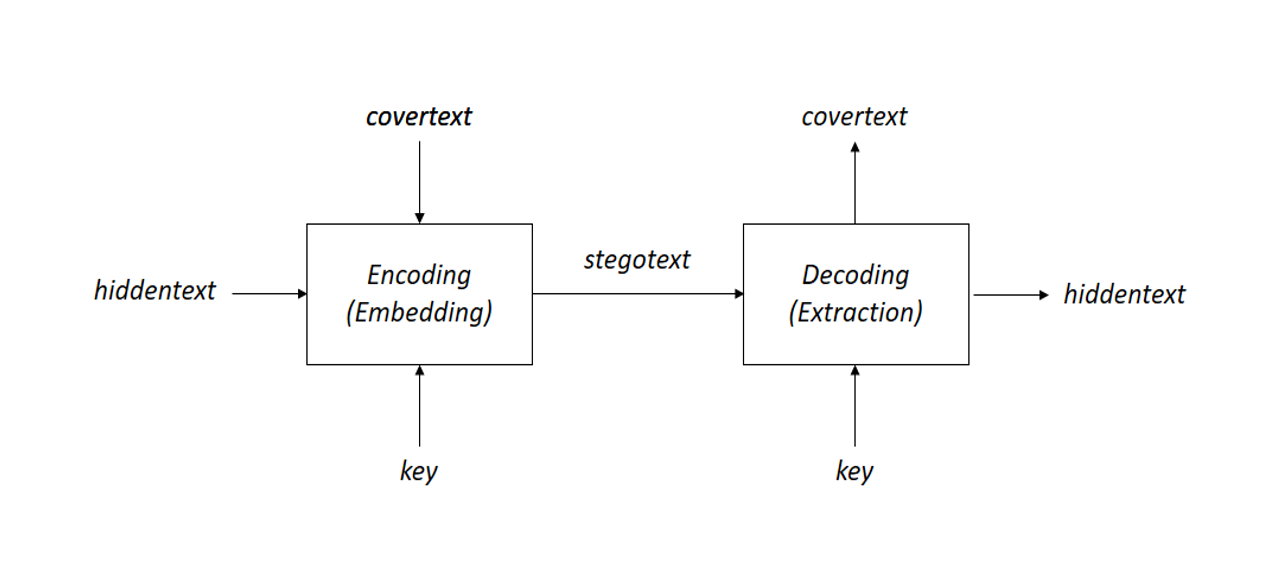
\includegraphics[width=1\textwidth]{gambar/diagram_steganografi}
		\caption{Diagram penyisipan dan ekstraksi pada pesan}
		\label{diagram_steganografi}
	\end{figure} 
	
	Istilah di dalam steganografi:
	\begin{enumerate}
		\item \emph{Covertext} merupakan media atau tempat pesan yang digunakan untuk menyembunyikan \emph{hiddentext}. \emph{Covertext} bisa berupa teks, gambar, audio, video, dll.
		\item \emph{Hiddentext}	atau biasa disebut \emph{embedded message} merupakan pesan atau informasi yang ingin disembunyikan. Contohnya bisa berupa teks, gambar, audio, video, dll.
		\item \emph{Stegotext} merupakan pesan yang sudah berisi \emph{embedded message}.
		\item \emph{Encoding} yaitu penyisipan pesan ke dalam media \emph{covertext}.
		\item \emph{Decoding} yaitu ekstraksi pesan dari \emph{stegotext}.
	\end{enumerate}
	
	Menurut \textbf{Munir}, ada kriteria yang harus diperhatikan dalam penyembunyian pesan, yaitu meliputi \emph{Imperceptible}, \emph{Fidelity}, \emph{Recovery} dan \emph{Capacity}.
	\begin{enumerate}
		\item \emph{Imperceptible}\\ 
		Keberadaan pesan rahasia tidak dapat dipersepsi secara visual atau secara audio. Jika \emph{covertext} berupa \emph{file} citra, maka \emph{stegotext} yang dihasilkan harus sukar dibedakan oleh kasat mata dengan \emph{covertext}-nya. Dan jika \emph{covertext} berupa \emph{file} audio, maka telinga tidak dapat mendeteksi perubahan yang ada pada audio \emph{stegotext}-nya. 
		\item \emph{Fidelity}\\
		Kualitas \emph{file} citra penampung tidak jauh berubah. Setelah penambahan pesan rahasia, citra hasil steganografi masih terlihat dengan baik. Pengamat tidak mengetahui kalau di dalam citra tersebut terdapat pesan rahasia.
		\item \emph{Recovery}\\
		Pesan yang disembunyikan harus dapat diekstrak kembali. Karena tujuan steganografi adalah menyembunyikan pesan atau informasi, maka jika informasi itu dibutuhkan harus dapat diambil kembali untuk dapat digunakan.
		\item \emph{Capacity}\\
		Ukuran pesan yang akan disembunyikan sedapat mungkin besar. Agar dapat memaksimalkan manfaat dari steganografi itu sendiri. \cite{munir}
	\end{enumerate}
	
	\subsection{Sejarah Steganografi}
	Seperti kriptografi, penggunaan steganografi sebetulnya telah digunakan berabad-abad yang lalu bahkan sebelum istilah steganografi itu sendiri muncul. Periode sejarah steganografi dapat dibagi menjadi:
	\begin{enumerate}
		\item Steganografi Kuno (\emph{Ancient Steganography})
			\begin{enumerate}
				\item Steganografi dengan media kepala budak
				
				Ditulis oleh \textbf{Herodatus} (485–525 BC), sejarawan Yunani pada tahun 440 BC di dalam buku: \emph{Histories of Herodatus}). Kisah perang antara kerajaan Persia dan rakyat Yunani. \textbf{Herodatus} menceritakan cara \textbf{Histaiaeus} mengirim pesan kepada \textbf{Aristagoras of Miletus} untuk melawan Persia. 
				
				Caranya adalah dengan dipilih beberapa budak. Kemudian kepala budak tersebut digunduli dan ditulis pesan dengan cara ditato. Setelah pesan dituliskan, budak harus menunggu hingga rambutnya tumbuh kembali. Setelah rambut pada kepala budak tersebut tumbuh, budak dikirim ke tempat penerima. Di sana kepala budak digunduli agar pesan dapat dibaca.
					\begin{figure}[H]
						\centering
						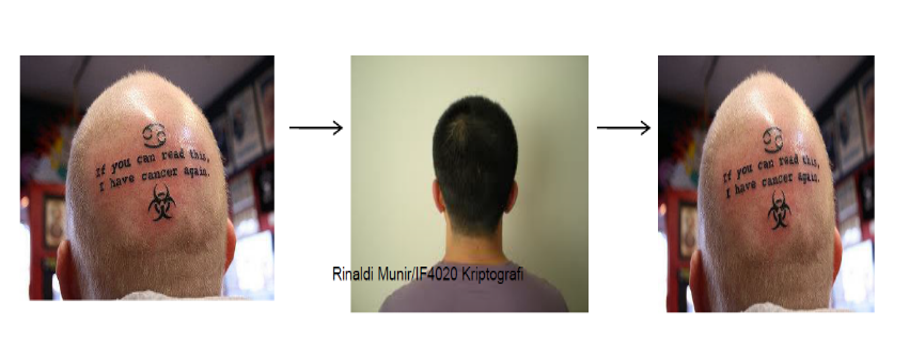
\includegraphics[width=1\textwidth]{gambar/steganografi_kepalabudak}
						\caption{Steganografi dengan media kepala budak}
						\label{steganografi_kepalabudak}
					\end{figure}
				
				\item Penggunaan tablet \emph{wax}
				
				Orang-orang Yunani kuno menulis pesan rahasia di atas kayu yang kemudian ditutup dengan lilin (\emph{wax}). Di dalam bukunya, \textbf{Heradatus} menceritakan \textbf{Demaratus} mengirim peringatan tentang serangan yang akan datang ke Yunani dengan menulis langsung pada tablet kayu yang kemudian dilapisi lilin dari lebah.
					\begin{figure}[H]
						\centering
						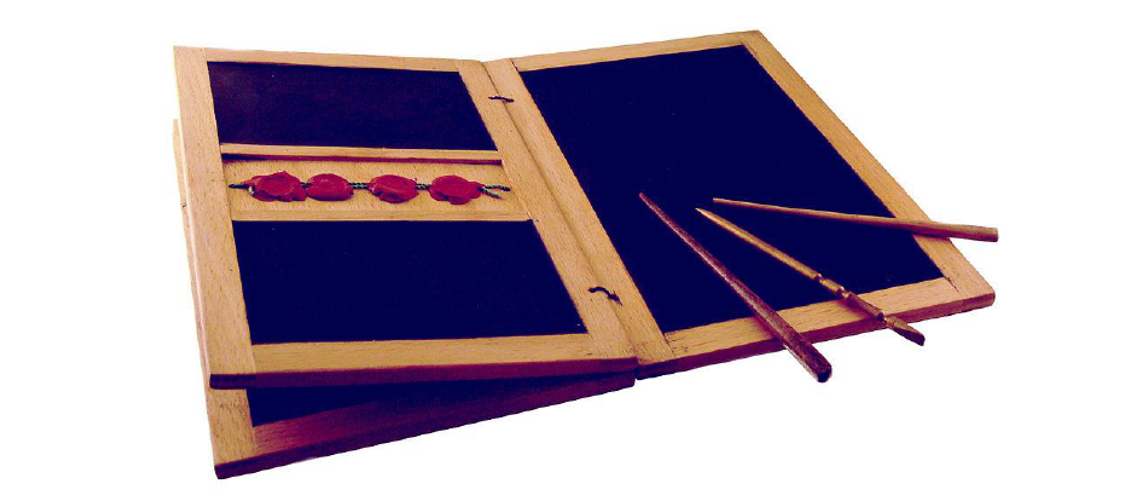
\includegraphics[width=1\textwidth]{gambar/tablet_wax}
						\caption{Tablet \emph{wax}}
						\label{tablet_wax}
					\end{figure}
					
				\item Penggunaan tinta tak-tampak (\emph{invisible ink})
				
				\textbf{Pliny the Elder} menjelaskan penggunaan tinta dari getah tanaman \emph{thithymallus}. Jika dituliskan pada kertas maka tulisan dengan tinta tersebut tidak kelihatan, tetapi bila kertas dipanaskan berubah menjadi gelap/coklat.
				
				\item Penggunaan kain sutra dan lilin
				
				Orang Cina kuno menulis catatan pada potongan-potongan kecil sutra yang kemudian digumpalkan menjadi bola kecil dan dilapisi lilin. Selanjutnya bola kecil tersebut ditelan oleh si pembawa pesan. Pesan dibaca setelah bola kecil dikeluarkan dari perut si pembawa pesan.			
			\end{enumerate}
		\item Steganografi Zaman Renaisans (\emph{Renaissance Steganography})
		
		Tahun 1499, \textbf{Johannes Trithemius} menulis buku \emph{Steganographia}, yang menceritakan tentang metode steganografi berbasis karakter. Selanjutnya tahun 1518 dia menulis buku tentang steganografi dan kriptografi berjudul \emph{Polygraphiae}.
		
		\textbf{Giovanni Battista Porta} menggambarkan cara menyembunyikan pesan di dalam telur rebus. Caranya, pesan ditulis pada kulit telur yang dibuat dari tinta khusus yang dibuat dengan satu ons tawas dan setengah liter cuka. Prinsipnya penyembunyiannya adalah tinta tersebut akan menembus kulit telur yang berpori, tanpa meninggalkan jejak yang terlihat. Tulisan dari tinta akan membekas pada permukaan isi telur yang telah mengeras (karena sudah direbus sebelumnya). Pesan dibaca dengan membuang kulit telur.
		
		\item Steganografi Zaman Perang Dunia (\emph{World War Steganography})
		
		\begin{figure}[H]
			\centering
			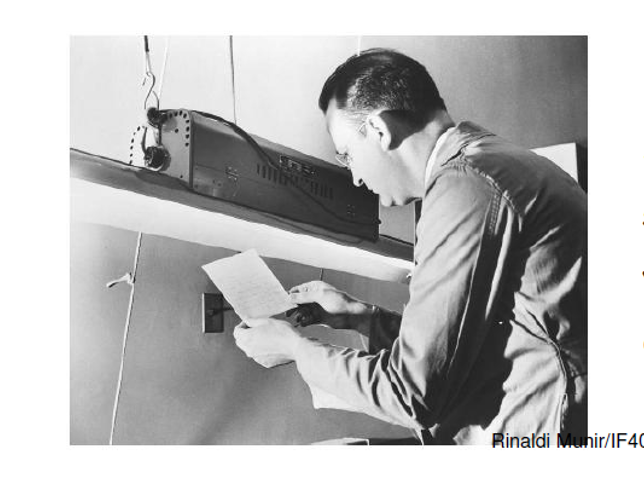
\includegraphics[width=1\textwidth]{gambar/steganografi_perangdunia}
			\caption{Steganografi zaman perang dunia}
			\label{steganografi_perangdunia}
		\end{figure}
	
		Selama terjadinya Perang Dunia ke-2, tinta yang tidak tampak (\emph{invisible ink}) telah digunakan untuk menulis informasi pada lembaran kertas sehingga saat kertas tersebut jatuh di tangan pihak lain hanya akan tampak seperti lembaran kertas kosong biasa. Cairan seperti air kencing (\emph{urine}), susu, vinegar, dan jus buah digunakan sebagai media penulisan sebab bila salah satu elemen tersebut dipanaskan, tulisan akan menggelap dan tampak melalui mata manusia. \cite{munir}
		
		\item Steganografi \emph{Digital}
		
		Sejalan dengan perkembangan maka konsep awal steganografi diimplementasikan pula dalam dunia komputer, yang kemudian dikenal dengan istilah steganografi \emph{digital}. Dalam hal ini, steganografi \emph{digital} memiliki dua properti dasar yaitu media penampung (\emph{cover data} atau \emph{data carrier}) dan data \emph{digital} yang akan disisipkan (\emph{secret data}), dimana media penampung dan data \emph{digital} yang akan disisipkan dapat berupa \emph{file} multimedia (teks/dokumen, citra, audio maupun video). Terdapat dua tahapan umum dalam steganografi \emph{digital}, yaitu proses \emph{embedding} atau \emph{encoding} (penyisipan) dan proses \emph{extracting} atau \emph{decoding} (pemekaran atau pengungkapan kembali (\emph{reveal})). Hasil yang didapat setelah proses \emph{embedding} atau \emph{encoding} disebut \emph{stego object} (apabila media penampung hanya berupa data citra maka disebut \emph{stego image}). \cite{prayudi}
	\end{enumerate}

	\subsection{Metode Steganografi}
	Berdasarkan ranah operasinya, metode-metode steganografi dapat dibagi menjadi dua kelompok:
	\begin{enumerate}
		\item \emph{Spatial (time) domain methods}\\
		Memodifikasi langsung nilai byte dari \emph{cover-object} (nilai \emph{byte} dapat merepresentasikan intensitas/warna \emph{pixel} atau amplitudo). Contoh: Metode modifikasi LSB
		
		\item \emph{Tranform domain methods}\\
		Memodifikasi hasil transformasi sinyal dalam ranah transform (hasil trnasformasi dari ranah spasial ke ranah lain (misalnya ranah frekuensi). Contoh: Metode \emph{Spread Spectrum} \cite{munir}
		
	\end{enumerate}

	Ada empat jenis metode steganografi:
	\begin{enumerate}
		\item \emph{Least Significant Bit Insertion} (LSB)\\
		Metode yang digunakan untuk menyembunyikan pesan pada media \emph{digital} tersebut berbeda-beda. Contohnya, pada berkas \emph{image} pesan dapat disembunyikan dengan menggunakan cara menyisipkannya pada bit rendah atau bit yang paling kanan (LSB) pada data \emph{pixel} yang menyusun \emph{file} tersebut. Pada berkas \emph{bitmap} 24 bit, setiap \emph{pixel} (titik) pada gambar tersebut terdiri dari susunan tiga warna \emph{Red}, \emph{Green} dan \emph{Blue} (RGB) yang masing-masing disusun oleh bilangan 8 bit (\emph{byte}) dari 0 sampai 255 atau dengan format biner 00000000 sampai 11111111. Dengan demikian, pada setiap \emph{pixel} berkas \emph{bitmap} 24 bit kita dapat menyisipkan 3 bit data. 
		\item \emph{Algorithms and Transformation}\\
		\emph{Algoritma compression} adalah metode steganografi dengan menyembunyikan data dalam fungsi matematika. Dua fungsi tersebut adalah \emph{Discrete Cosine Transformation} (DCT) dan \emph{Wavelet Transformation}. Fungsi DCT dan \emph{Wavelet} yaitu mentransformasi data dari satu tempat (\emph{domain}) ke tempat (\emph{domain}) yang lain. Fungsi DCT yaitu mentransformasi data dari tempat \emph{spatial} (\emph{spatial domain}) ke tempat frekuensi (\emph{frequency domain}).
		\item \emph{Redundant Pattern Encoding}
		\emph{Redundant Pattern Encoding} adalah menggambar pesan kecil pada kebanyakan gambar. Keuntungan dari metode ini adalah dapat bertahan dari \emph{cropping} (kegagalan). Kerugiannya yaitu tidak dapat menggambar pesan yang lebih besar.
		\item \emph{Spread Spectrum Method}
		\emph{Spread Spectrum} steganografi terpencar-pencar sebagai pesan yang diacak (\emph{encrypted}) melalui gambar (tidak seperti dalam LSB). Untuk membaca suatu pesan, penerima memerlukan algoritma yaitu \emph{crypto-key} dan \emph{stego-key}. Metode ini juga masih mudah diserang yaitu penghancuran atau pengrusakan dari kompresi dan proses \emph{image} (gambar)	
	\end{enumerate}

\section{Perbedaan Steganografi dan Kriptografi}
\section{LSB (\emph{Least Significant Bit})}
\section{ASCII}
\section{\emph{Citra Digital}}
	\subsection{Pengertian Citra \emph{Digital}}
	\subsection{Pengolahan Citra \emph{Image Processing}}
	\subsection{Perbandingan \emph{File} Gambar BMP (\emph{Bitmap}) dengan JPG, GIF, atau PNG}
\section{MATLAB}	



% Baris ini digunakan untuk membantu dalam melakukan sitasi
% Karena diapit dengan comment, maka baris ini akan diabaikan
% oleh compiler LaTeX.
\begin{comment}
bibliography{daftar-pustaka}
\end{comment}
